\documentclass[a4paper,12pt]{article}
\usepackage[utf8]{inputenc}
\usepackage{fullpage}
\usepackage[style=phys,maxbibnames=6]{biblatex}
\usepackage[skip=0em,indent=2em]{parskip}
\usepackage[pdftex]{graphicx}
\usepackage{float}
\usepackage{caption}
\usepackage{subcaption}
\usepackage{hyperref}
\usepackage{physics}
\usepackage{amsmath}
\usepackage{siunitx}
\usepackage{fancyvrb}
\usepackage{cleveref}
\usepackage{duckuments}
\usepackage[toc,page]{appendix}


\addbibresource{references.bib}

\DeclareMathOperator{\diag}{diag}
\DeclareMathOperator{\Gaus}{Gaus}

\AtBeginEnvironment{appendices}{\crefalias{section}{appendix}}

% My newcommands to save typing
\newcommand{\efn}{e4$\nu$}
\newcommand{\eGEN}{$e\text{-GENIE}$}

\newcommand{\verbb}[1]{\text{\Verb|#1|}}

\newcommand{\Mu}{$\mu$}
\newcommand{\Tau}{$\tau$}

\newcommand{\Ne}{$\nu_e$}
\newcommand{\Nm}{$\nu_\mu$}
\newcommand{\Nt}{$\nu_\tau$}

\newcommand{\Zz}{$Z^0$}
\newcommand{\Wp}{$W^+$}
\newcommand{\Wm}{$W^-$}
\newcommand{\Wpm}{$W^\pm$}
\newcommand{\pip}{$\pi^+$}
\newcommand{\pim}{$\pi^-$}

\newcommand{\md}{$1\pi^-1p$}
\newcommand{\pd}{$1\pi^+1n$}

\newcommand{\duckim}[2][0.8]{
    \begin{figure}[H]
        \centering
        \includegraphics[width=#1\textwidth]{example-image-duck}
        \caption{
            Ducky: #2
        }\label{fig:nu_fen}
    \end{figure}
}

\begin{document}
\pagestyle{empty}
\par\noindent
\includegraphics[width=12cm]{PandA_crest.pdf}
\par\noindent

\vspace*{2cm}

\begin{center}
        \Large\bf \Large\bf Senior Honours Project \\
        \LARGE\bf Further analysis of \efn\ data
\end{center}

\vspace*{0.5cm}

\begin{center}
        \bf Jan Kocka \\
        February 2022
\end{center}
\vspace*{5mm}

\begin{abstract}
    \noindent
    This report outlines the need for a better understanding of neutrino-nucleus interactions and how studying electron-nucleus interaction can be just as illuminating as working directly with neutrinos.
    It covers some of the prerequisites to understand such studies, including the most commonly studied interaction types and the use of Monte Carlo event generators like GENIE.
    An introduction to the CLAS6 data used by the \efn\ collaboration is presented and a new codebase using modern C\texttt{++} to analyse the data was developed.
    Finally we use this code to conduct a study of nuclear effects on the reconstruction of pion momentum of 1 pion 1 nucleon events (mainly from $\Delta_{1232}$ resonances) from GENIE generated 2.26\si{GeV} incident electron - carbon nucleus scattering.
    We identify errors of the reconstruction due to initial state effects and final state interactions, however even once adjusting for detector precision reconstructing pion momentum should be possible within 400 \si{Mev/c}.
\end{abstract}

\vspace*{1cm}

\begin{center}
    \textbf{\normalsize Declaration}

      I declare that this project and report is my own work.
\end{center}

\vspace*{4cm}
Signature:\hfill Date:  31/3/2023

\vfill
{\bf Supervisor:} Dr. Cheryl Patrick
\hfill
Completed in 10 Weeks
\newpage

\tableofcontents

\newpage

\pagestyle{plain}
\setcounter{page}{1}

\section{Neutrino Oscillations and Understanding Neutrino Scattering}
This project concerns neutrinos and their properties, and so a brief description of the relevant properties and their scientific significance is presented.
Neutrinos are three uncharged leptons of different flavours (each corresponding to the other 3, charged, leptons -- electron, \Mu\ and \Tau\ of ascending masses).
Neutrinos interact only via the weak force and with very low cross sections, the Feynman diagrams of their interactions with the other fundamental particles through the W and Z bosons are shown in \cref{fig:nu_feyn}.

Their existence was originally proposed by Pauli in the 1930s to explain the beta decay, and their mass was long thought to be 0, most notably the standard model assumes this.
However at the end of the last century neutrinos have been observed to undergo oscillations which implies non-zero mass.
Since then they have been at the forefront of research, nowadays they are accepted to have mass and there are questions about them being their own antiparticles (Majorana) and possibly violating charge-parity symmetry.
The answers to these questions could significantly further our understanding of the universe, including explaining the dominance of matter over antimatter.

\begin{figure}[H]
    \centering
    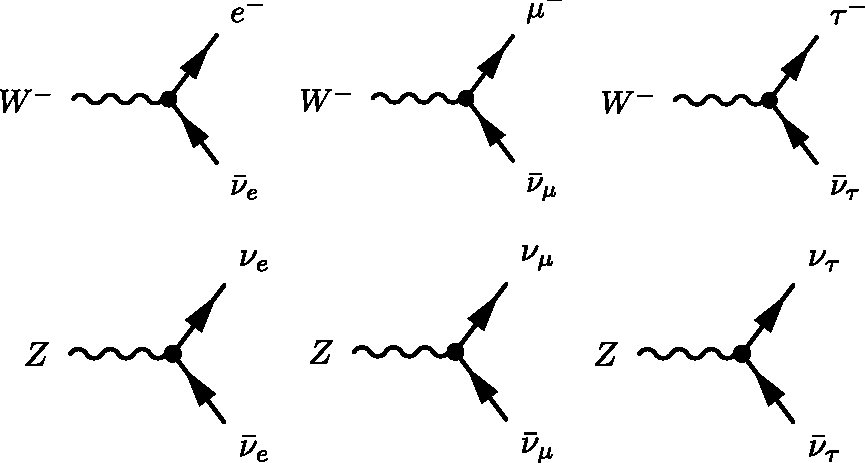
\includegraphics[width=0.55\textwidth]{figures/NeutrinoFeynman.pdf}
    \caption{
        Feynman diagrams of weak force vertices for neutrino interactions, all other vertices including them can be obtain by suitable rotations of these
        (this requires replacing some particles with their antiparticles, including the \Wm becoming a \Wp).
        Say the first could be changed to represent a $e^-$ and \Wp\ colliding and forming a \Ne.
        Diagrams taken from \cite{potterFeynmanDiagramsParticlea}.
    }\label{fig:nu_feyn}
\end{figure}

\subsection{Neutrino Oscillations}
In particle physics oscillations is a phenomenon that takes place when the particle mass eigenstates which govern its evolution in time are not the same as the state in which it is observed.
This phenomenon is not exclusive to neutrinos, the neutral Kaon has been known to oscillate to its own antiparticle and vice-versa since before neutrino oscillations were discovered \cite{burkhardtWavelengthNeutrinoNeutral2003}.
% However it might seem a bit abstract, but as we know from basic quantum mechanics when we make an observation, the observed system will collapse into some particular state depending on the result of our observation.

In the case of neutrinos, we say there are three flavours and the way we differentiate them is by the weak interaction, as so far all interactions we observed conserve the three separated lepton numbers (electron, \Mu\ and \Tau\ again).
So say an electron capture takes place when an electron interacts with a proton to form a neutron and a neutrino, then we observe that neutrino to be an electron neutrino in order to conserve the electron lepton number and we can say it is collapsed into the electron neutrino eigenstate.

Further, that electron eigenstate can be expressed in terms of the mass eigenstates, and if the two eigenstate sets aren't identical it will have multiple non-zero components.
Then as the mass eigenstates travel differently (the neutrino has a definite $E$ and so through $E^2 = m^2 + p^2$ we get that the mass eigenstates have different momenta and so speeds), the relative components of the state at different positions as it travels will change periodically -- oscillate.
Thus the probabilities of measuring the neutrino in any of the three flavour states also oscillates.
% The result is that if a neutrino is measured to be of some known flavour the probability of measuring it at a later time in any of the other flavour states changes and it might later be measured to be of a different flavour.

A very important property resulting from the two eigenstate sets being different is the transformation matrix between them.
For neutrinos this is the PMNS\footnotemark\ matrix, it is referred to as $U$ and is such that 
\begin{equation}
    \ket{\nu_\alpha} = \sum_i U_{\alpha i} \ket{\nu_i}, \text{ and }
    \ket{\nu_i} = \sum_\alpha U^\dag_{i \alpha} \ket{\nu_\alpha}
\end{equation}
where $\ket{\nu_\alpha}$ are the three flavour eigenstates and $\ket{\nu_i}$ the mass eigenstates.
The exact form of the matrix then determines many of the neutrino properties, obtaining accurate values for its elements is the main driving force of neutrino oscillation experiments.
For example if the matrix is not completely real then neutrinos violate CP symmetry.
\footnotetext{Stands for Pontecorvo–Maki–Nakagawa–Sakata matrix, it is the analogue of the CKM matrix for the mixing of quarks.}

Then to complete the picture, the probability of a neutrino measured to be of flavour $\alpha$, to be measured again in the flavour $\beta$ is given by 
\begin{equation} \label{eq:nosc}
    P(\alpha \rightarrow \beta) = \sum_i |U_{\alpha i} U^\dag_{i \beta}|^2 + 2\Re \sum_{j>i} U_{\alpha i} U^\dag_{i \beta} (U_{\alpha j} U^\dag_{j \beta})^* \exp(-i\frac{\Delta m^2_{ij}}{2}\frac{L}{E})
\end{equation}
where $E$ is it's energy, $L$ the distance between our measurements and $\Delta m^2_{ij}$ the mass difference of the mass eigenstates $i, j$ squared (for more detail see \cite{zuberNeutrinoPhysics2020}).
This is then our main entry point for studying the PMNS matrix from oscillation experiments as we can measure these probabilities $P$ and deduce some of the values or their relations along with the mass differences $\Delta m_{ij}$.
Though even if we  knew precisely all the oscillation probabilities we still can not fully determine the matrix, there may be a Majorana phase component that doesn't influence $P$ and so needs to be studied using other experiments.

\subsection{Oscillation Experiments and Energy Reconstruction}\label{sec:exanderec}
There are many active experiments (NOvA and T2K currently running and DUNE and Hyper-Kamiokande under development) working on precise neutrino oscillation measurements to determine the neutrino masses and PMNS matrix elements.
% There are active experiments (including Super-Kamiokande, OPERA, MINOS, DUNE and Hyper-Kamiokande\footnote{**maybe change which ones I mention and add references to them}) working on precise neutrino oscillation measurements to determine the neutrino masses and PMNS matrix elements.
In these (long-baseline) experiments, neutrinos from a source which has known fractions of the three flavours are beamed across large distances (for oscillations of $\sim 1\si{GeV}$ \Nm\ an $L$ of order $\sim 1000\si{km}$ is needed \cite{mezzettoThreeFlavorOscillationsAccelerator2020}) so that they oscillate and then some of the flavours (electron, \Mu\ or both) are observed and counted.
This means we are measuring some of the probabilities from \cref{eq:nosc} with a known $L$, however we don't have a simple value for $E$ which we need in order to interpret the data.
Experiments typically use either neutrinos from the sun, from the atmosphere due to the cosmic microwave background or from secondary neutrino beams at accelerators and all of these methods produce neutrinos with wide ranges of energies (see \cref{fig:neu_s_Es}).
Because of that experiments rely on reconstructing incident neutrino energies and for that a very good understanding of the detecting mechanism is needed.

\begin{figure}[H]
    \centering
    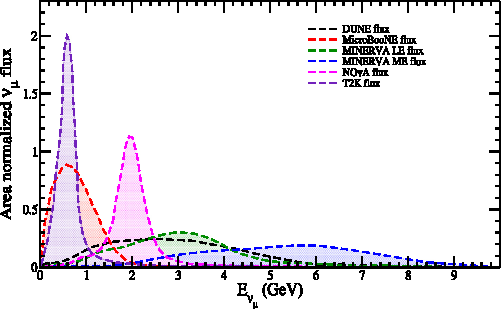
\includegraphics[width=0.6\textwidth]{figures/sourceEnergies.pdf}
    \caption{
        The energy distributions of neutrino sources used at various experiments, both oscillation (DUNE, NOvA, T2K) and neutrino interaction studies (MicroBooNE, MINERVA).
        All of these are accelerator based sources which have the narrowest energy distributions, however still the spread is on the order of hundreds of \si{MeV} at least.
        Figure taken from \cite{sajjadatharNeutrinosTheirInteractions2023}.
    }\label{fig:neu_s_Es}
\end{figure}

As neutrinos are uncharged and have tiny cross sections, they aren't detected directly, instead a large amount (needed due to the small cross sections) of some stable substance (argon, water or chlorine) is stored and surrounded by detectors (often carbon based scintillators).
Then when neutrinos come in, some will interact with these atoms and produce detectable particles.
These always have to include a lepton of the corresponding flavour and possibly other particles, often nucleons, photons or pions and a collection of particle measurements originating from one neutrino is called an event.
While the neutrinos can interact with the atomic electrons \cite{whittinghamScatteringLowEnergy2022}, it is only significant at low neutrino energies and rarely relevant to oscillation experiments.
Thus some of the most important physics of neutrino detectors are the neutrino-nucleus interactions and these are not yet well understood.
Modern oscillation experiments report these limitations to be a source of large systematic uncertainties\cite{abeConstraintMatterAntimatter2020,novacollaborationNewConstraintsOscillation2018}.

\subsection{\efn\ and nuclear effects}
Which is where \efn\ comes in, while ideally we would study these interaction with neutrinos, but the absence of a monoenergetic neutrino source, along with their small cross sections makes us consider other options.
While on the surface it may seem different, electrons scatter off of nuclei in a similar manner, and further, nuclear effects are identical.
Nuclear effects mainly come in two flavours, initial state effects and final state effects.

Initial state nuclear effects describe how the state of the nucleus before the collision affects our measurements.
An example demonstrated later on is that if the incident lepton scatters a nucleon outside the nucleus and we want to use 4 momentum conservation for analysis, we need to account for the 4 momentum of the original nucleon, and possibly the nucleus within the sample, neither of which are simple to model.

However, likely more problematic are Final State Interactions (FSI), these can occur when the first (primary) lepton interaction creates or scatters other hadrons, which happens nearly always.
These hadrons then start within the nucleus and can interact with it before escaping it.
This is a significant effect, for $\sim 1\si{GeV}$ neutrinos impacting an iron target, about 30\% of the created hadrons undergo FSI\cite{stevendytmanFinalStateInteractions2009}.
FSI can not only change the particle 4 momentum but also result in particle creation or absorption, completely changing the composition of the particles we detect.
See \cite{golanEffectsFinalstateInteractions2012,stevendytmanFinalStateInteractions2009} for more detail.

% further after the first neutrino-nucleus interactions, the resulting hadrons will often interact with each other too.
% This is called Final State Interactions (FSI) or nuclear effects, these are very relevant to oscillation experiments as they significantly change the resulting particles we detect and they are identical for neutrino and electron-nucleus scattering.
% So in summary, we can use easily available electron scattering data to test neutrino interaction models -- \efn.

% in order to better interpret data from neutrino detectors and mainly to improve their energy reconstruction (which is becoming a significant factor on the uncertainties of the results) we need to understand these neutrino-nucleus interactions better.

% However, as there are no monoenergetic neutrino beams it is very difficult to experimentally study these effects directly on neutrinos, so instead we study electron-nucleus interactions which are subject to the same quantum field theory interactions.

\section{Neutrino(Electron)-nucleus interactions}
Firstly, throughout the report antineutrinos are largely not mentioned, their interaction do have some specifics to them, however are mostly directly analogous to the described neutrino processes.
As the interactions are not yet fully, fundamentally understood, we to a large degree resort to classifications which allows us to make prediction under certain conditions.
Both neutrino and electron nucleus scattering can be described by
\begin{equation}\label{eq:genint}
    l + A \rightarrow l' + a + b + c ...
\end{equation}
where an incoming lepton $l$ scatters off of a nucleus $A$ resulting in a lepton $l'$ and hadron particles $a, b, c ...$.
When considering realistic experiments we always know $l$ and $A$ but might only be able to detect the outgoing lepton and some or none of the outgoing hadrons. 
To differentiate these cases we consider separately \emph{inclusive} cross sections where only $l'$ is detected (so the result is essentially as if summing over all the possible outgoing hadrons).
\emph{Semi-inclusive} cross sections where $l'$ and some of the hadrons are detected and \emph{exclusive} cross sections where we know all of the resulting particles \cite{amaroElectronNeutrinonucleusScattering2020}.

As neutrinos only interact via the weak force, all neutrino-nucleus interactions take place via either the \Zz\ boson, in which case the final lepton is the same neutrino.
These are called \emph{Neutral Current} (NC) events and are generally difficult to measure as we cannot measure the outgoing lepton and have to rely on reconstructing the event solely from the hadrons \cite{giustiNeutralCurrentNeutrinonucleus2020}.
Or it can interact through the \Wp and \Wm\ bosons (\emph{Charged Current} or CC interactions) in which case a charged lepton is produced and detected, often being the most important particle for detection and event reconstruction.

This is contrasted to electrons which will dominantly interact with the nucleus through photons (so preserving the electron).
Nevertheless within quantum field theory the neutrino weak force interactions have a vector and an axial-vector components and the electron EM interaction has only a vector component\cite{alvarez-rusoNuSTEC11NeutrinoScattering2018}.
Thus, the vector part of neutrino-nucleus scattering calculations and simulations can be adapted and tested by electron scattering.
% Due to this existing MC event generators like GENIE can be modified to generate electron-nucleus interaction events and test particularly the vector current component of the theories behind the generator.
% Further on I will only speak about neutrino interactions, but most of these characteristics apply to electrons too.


\subsection{Particle and event properties}
This is also a good place to introduce some ways in which we describe events and the particles in them.
As these are high energy particles, we have to treat them relativistically, as such the key property of a particle is its 4 momentum $p^\mu$, or equivalently energy $E$ and relativistic 3 momentum $\vb{p}$.
For our coordinate systems we choose the incident particle beam direction to be along the Cartesian $e_z$ and we often use spherical polars with respect to this axis and such that $\theta = 0$ corresponds to $e_z$ (often $\cos{\theta}$ is used instead of $\theta$).
The specific orientation of $e_x$ and $e_y$ isn't very important and so is mostly glossed over, in addition we use natural units in which $\hbar = c = 1$ and in the report we write 4 vectors such that the SR metric $\eta_{\mu \nu}$ is $\diag(1, -1, -1, -1)$ (though notably GENIE, ROOT, see \cref{sec:genie}, and so our data uses a convention where it is $\diag(-1, -1, -1, 1)$).
For example this means an incident particle of mass $m$ and energy $E$ would have
\begin{equation}
    q_i^\mu \leftrightarrow \begin{pmatrix} E \\ \sqrt{E^2 - m^2} \\ 0 \\ 0 \end{pmatrix}
\end{equation}

In the events we consider, we have an incident lepton with 4 momentum $q_{i}^\mu$ impacting the nucleus and let $p_i^\mu$ be the outgoing leptons 4 momentum.
A very common scattering property within particle physics is the 4 momentum transfer $q^2$, here it is the 4 momentum change of the incident particle squared, so $(p_i^\mu - q_i^\mu)^2$, though within neutrino interactions typically $Q^2 = -q^2$ is used instead.
Next, there is $W^2$, the invariant mass of all the produced hadrons, with regard to \cref{eq:genint}, one of $a, b, c \ldots$ will be the remaining nucleus and $W^2 = r_\mu r^\mu$ where $r^\mu$ is the total 4 momentum of all the others.
% Notably that means we can reconstruct $W$ using only electron 4 momentum, assuming the struck nucleon was at rest as then .
% This is not a completely valid assumption, however it can lead to good results
There are other common event properties, notably the Bjorken scaling variables $x, y$, however they are not of interest in this report.

\subsection{Interaction types}
\begin{figure}[H]
    \centering
    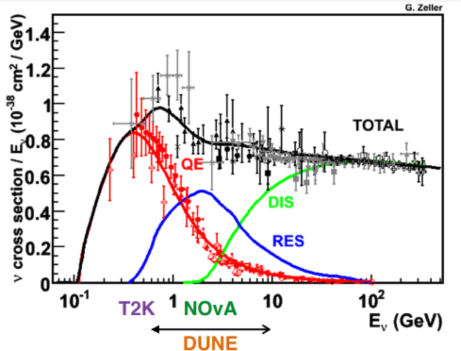
\includegraphics[width=0.6\textwidth]{figures/sigmaVsEnu.pdf}
    \caption{
        The differential cross section of neutrino-nucleus interactions shown for different interaction mechanisms and their sum.
        Near the x axis the approximate regions of interests for the T2K, NOvA and DUNE experiments is shown.
        Figure originally from \cite{formaggioEVEeVNeutrino2012}.
    }\label{fig:nusigma_vs_Enu}
\end{figure}

Finally to come back to the interaction types mentioned in \cref{sec:exanderec}, some of the main types relevant for oscillation experiments are Quasi-Elastic (QE), Resonant (RES) and Deep Inelastic Scattering (DIS), see \cref{fig:nusigma_vs_Enu}.
In this order these dominate at increasing energies and correspond with how far inside the nucleus the neutrino penetrated.
Importantly, these classifications also carry over to electron scattering very well, in fact they are referred to within neutrino physics under the same names, even though QE electron scattering is much closer to fully elastic scattering.
% A low energy neutrino ($<1\si{GeV}$) will scatter off of a nucleon as a whole, without changing it's composition.
% At medium energies ($\sim 1 \si{GeV}$) the neutrino can excite a nucleon into an excited state and at the highest energies ($>3\si{GeV}$) the neutrino will interact with many particles and DIS interactions become difficult to predict especially once accounting for FSI.

\subsubsection{Quasi-Elastic (QE) scattering}
Elastic scattering refers to processes where the internal structure of the colliding objects isn't altered.
Fully elastic neutrino scattering can then only happen within NC interactions.
However, there is a very similar CC interaction where the neutrino interacts with a single neutron through an $W$ boson, changing it into a proton, but otherwise conserving it's structure.
This is shown in \cref{fig:QE_fd} and as mentioned before these dominate at lower neutrino energies ($< 1\si{GeV}$).
In many ways they are the simplest interaction as they don't require as much information about that nucleus theoretically and experimentally they have a very clear signature of one electron and one nucleon with FSI not playing a major role.

\begin{figure}[H]
\centering
    \begin{subfigure}[b]{0.45\textwidth}
        \centering
        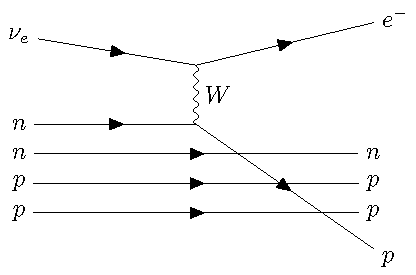
\includegraphics{figures/fds/QEFDneu.pdf}
        \caption{
            One of the neutrons is converted to a proton and scattered outside the nucleus (making the nucleus a Helium 3).
        }
    \end{subfigure}
    \hspace{1em}
    \begin{subfigure}[b]{0.45\textwidth}
        \centering
        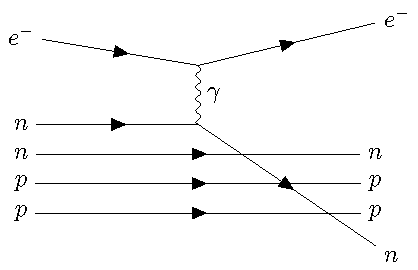
\includegraphics{figures/fds/QEFDel.pdf}
        \caption{
            Here the electron only scatters one of the neutrons (or protons) out of the nucleus but it remains the same type.
        }
    \end{subfigure}
    \caption{
        A Feynman diagrams of typical QE interactions of an electron neutrino and an electron with a Helium 4 nucleus.
        (The $W$ boson can be positive of negative depending on the time ordering.)
    }\label{fig:QE_fd}
\end{figure}

Of the neutrino interactions, QE are the best theoretically understood, the simplest models rely on a combination of two independent parts: calculations of neutrino-nucleon interactions within the impulse-approximation and modelling of the nucleons within the nuclei.
A recent review \cite{gallagherNeutrinoNucleusInteractions2011} has compared the theoretical result with observations from the MiniBooNE and NOMAD.
While the models capture many important features, there are also significant discrepancies which point to the interaction being more complicated than thought and also points out that many studies consider different levels of inclusiveness leading to difficulties in comparisons.

As they are not a focus of this work, we don't go further into detail, however it is worth saying that QE interactions are also a great example of the similarities of neutrino and electron scattering.
Theoretically, QE neutrino scattering is very similar to elastic electron scattering off of nucleons in nuclei (also referred to as QE) and as electrons have been studied earlier it has served as inspiration for the neutrino QE scattering theories.
Within \efn\ the same data this report will be working with has been inspected for testing incident electron energy reconstruction for QE scattering in \cite{khachatryanElectronbeamEnergyReconstruction2021}.

\subsubsection{Resonant scattering (RES) with focus on $\Delta$ and pion production}
Resonant interactions are dominant for neutrinos at energies near 1 \si{GeV}, they are the next logical step, the neutrino still only interacts with one nucleon, however this time that nucleon changes into an excited baryon state which promptly decays.
There are a couple possible such excited states, called \emph{resonances}, including various $N$ and $\Delta$ particles with spins $\frac{1}{2}, \frac{3}{2}$ or possibly more \cite{leitnerElectronNeutrinonucleusScattering2009}.
Here we focus on $\Delta_{1232}$ resonances (with masses near 1232 \si{MeV} and spin $\frac{3}{2}$, throughout the report $\Delta \sim \Delta_{1232}$) as they are are some of the most dominant and suitable to study as they decay into pion and nucleon pairs with a branching fraction of 99.4\% \cite{particledatagroupReviewParticlePhysics2022}.
Other processes are largely similar to these.

\begin{figure}[H]
    \centering
    \begin{subfigure}[b]{0.3\textwidth}
        \centering
        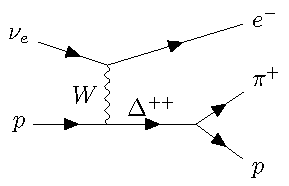
\includegraphics{figures/fds/RESneu1.pdf}
        \caption{
            $\pi^+pe^-$ final state
        }
    \end{subfigure}
    \begin{subfigure}[b]{0.3\textwidth}
        \centering
        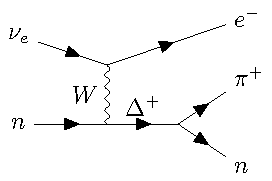
\includegraphics{figures/fds/RESneu2.pdf}
        \caption{
            $\pi^+ne^-$ final state
        }
    \end{subfigure}
    \begin{subfigure}[b]{0.3\textwidth}
        \centering
        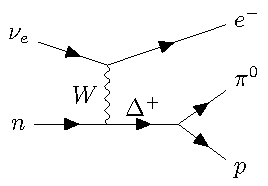
\includegraphics{figures/fds/RESneu3.pdf}
        \caption{
            $\pi^0pe^-$ final state
        }
    \end{subfigure}
    \caption{
        All possible CC $\Delta$ resonant electron neutrino scattering processes summarized, only showing the relevant nucleon, the rest form the remaining nucleus.
        The processes are identical for $\nu_\mu$ and $\mu_\tau$ except with the other leptons replacing the final state electron.
    }\label{fig:RES_fd}
\end{figure}

\begin{figure}[H]
    \centering
    \begin{subfigure}[b]{0.45\textwidth}
        \centering
        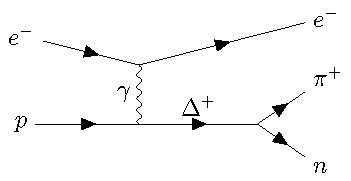
\includegraphics{figures/fds/RESel1.pdf}
        \caption{
            $\pi^+ne^-$ final state
        }
    \end{subfigure}
    \begin{subfigure}[b]{0.45\textwidth}
        \centering
        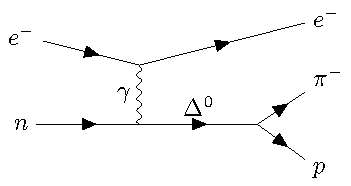
\includegraphics{figures/fds/RESel2.pdf}
        \caption{
            $\pi^-pe^-$ final state
        }
    \end{subfigure}

    \begin{subfigure}[b]{0.45\textwidth}
        \centering
        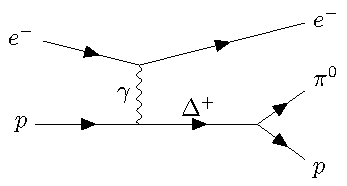
\includegraphics{figures/fds/RESel3.pdf}
        \caption{
            $\pi^0pe^-$ final state
        }
    \end{subfigure}
    \begin{subfigure}[b]{0.45\textwidth}
        \centering
        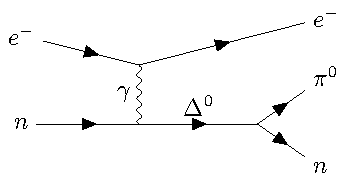
\includegraphics{figures/fds/RESel4.pdf}
        \caption{
            $\pi^0ne^-$ final state
        }
    \end{subfigure}
    \caption{
        $\Delta$ resonant electron scattering processes, (b) and (a) are the most important for this project as our data includes detected charged pions and protons.
    }\label{fig:RESel_fd}
\end{figure}

The CC $\Delta$ resonant processes for neutrino scattering are shown in \cref{fig:RES_fd} where only the struck nucleon is shown, the others are unaffected and form the post-collision nucleus.
NC processes are analogous and summarized as
\begin{align}
    \nu + p &\rightarrow \nu + \pi^+ + n & \nu + n &\rightarrow \nu + \pi^- + p \\
    \nu + p &\rightarrow \nu + \pi^0 + p & \nu + n &\rightarrow \nu + \pi^0 + n
\end{align}
and finally, the equivalent electron scattering processes are shown in \cref{fig:RESel_fd}.

Resonant interactions are often studied as they are in many ways the next step in complexity after QE events and one of their distinctive features is pion production.
This is important as pions can be detected by scattering experiments, though while charged pions have a mean lifetime of $\sim 10^{-8} \si{s}$, enough to reach a detector.
$\pi^0$ have lifetimes of $\sim 10^{-17} \si{s}$ \cite{particledatagroupReviewParticlePhysics2022} and decay into two photons before detection, they can then be reconstructed from photon measurements, however that adds complexity and so in this report we only look at charged pion events.

Other than RES interactions, pions can also be produced by coherent pion production where the neutrino/electron scatters off of the whole nucleus \cite{sogarwalCoherentPionProduction2022,higueraMeasurementCoherentProduction2014} however these mostly dominated by the other processes at higher energies.
Further pions can also be produced in FSI by any interaction type or in DIS interactions before FSI, however both of these processes can create many particles at once and so are very difficult to work with.
For these reasons in our analysis we try to restrict the amount of these events in our sample, so that we can focus on simple pion production where the kinematics can be understood.

\subsubsection{Deep Inelastic scattering (DIS)}
Finally at high energies ($>3\si{GeV}$) DIS events start to dominate.
In these the neutrino no longer interacts with a whole nucleon but some quark within a nucleon or a "sea" quark

\subsection{The GENIE Event Generator \cite{andreopoulosGENIENeutrinoMonte2010}}\label{sec:genie}
Due to the amount expertise required to understand either the theory or the experimental aspects of neutrino interactions, it becomes difficult to package theories in a way that they can be easily understood and tested by experiments.
Partly due to this the Neutrino Scattering Theory-Experiment Collaboration (NuSTEC \cite{alvarez-rusoNuSTEC11NeutrinoScattering2018}) has been started recently.
As a result, Monte Carlo (MC) neutrino event generators are often used to package theoretical models in a way that predictions can be made.
GENIE is the most widely adopted such MC generator, first released for use in 2007 it aims to be a canonical generator accurately reflecting the state-of-art theories for a wide range of energies and targets.
It is a large codebase of modern C\texttt{++} code using the popular ROOT libraries\cite{brunROOTObjectOriented1997} and is particularly well tuned to a tested on the few \si{GeV} energy neutrinos that are of interest to oscillation experiments.

As is described in \cite{andreopoulosGENIENeutrinoMonte2010}, there are three main categories of models in GENIE.
Nuclear physics models model the nuclei and their composition, this strongly depends on the energy of the incoming neutrino and whether it will scatter mostly off of a whole nucleon or a quark.
GENIE uses a Relativistic Fermi Gas (RFG) model for this step which is particularly successful at lower energies.
Then cross sections are calculated for various scattering types using their cross-section models and one is randomly chosen according to these.
These types include the ones mentioned above, but they are both further divided and other interactions are considered, including NC scattering and neutrino-electron scattering.
Hadronization models then finalize the primary interaction by predicting which hadrons are produced, for these GENIE uses the AGKY model from the MINOS experiment \cite{HadronizationModelMINOS}.
However, for many of these there are options of models to choose from, two main tuning setups used in \efn\ are the G2018 (somewhat more empirical separating the different interactions earlier) and GSuSAv2, which we use here, this uses a super-scaling lepton scattering model\cite{amaroNeutrinonucleusScatteringSuSA2021}.

% As has been mentioned before within QFT a large amount of the models for neutrino scattering are the same for electrons and these have been directly adapted within GENIE to create \eGEN, a mode of operation that can simulate electron-nucleus scattering events.
% \eGEN\ has been revised in 2021 by the \efn\ collaboration \cite{e4ncollaborationInclusiveElectronScattering2021} and is really at the core of the project.
% Data from it, including the data used in this report, can then be studied and compared to experimental data.
GENIE also has an electron scattering mode (\eGEN) that has been revised in 2021 by the \efn\ collaboration \cite{e4ncollaborationInclusiveElectronScattering2021}.
This uses the same underlying logic and structures of GENIE, as mentioned before within QFT both neutrino and electron interactions have a vector component, so that part of the code is reused.
\eGEN\ is then use to generate electron scattering data to test the underlying models.

\section{The \efn\ CLAS6 Data and Writing the Analysis Code}
The data used by the \efn\ analysis comes from the e2a experiment measuring electron scattering at electron energies of 1.16, 2.26 and 4.45 \si{GeV} on targets of He, C and Fe nuclei.
The measurements took place in Thomas Jefferson National Accelerator Facility (JLab) using the CEBAF Large Acceptance Spectrometer (CLAS6) \cite{meckingCEBAFLargeAcceptance2003} in 1999, the data has been used in many published works including \cite{khachatryanElectronbeamEnergyReconstruction2021}.
In addition, recently CLAS has undergone an upgrade (CLAS6 to CLAS12) \cite{burkertCLAS12SpectrometerJefferson2020} allowing experiments at electron energies up to 12 \si{GeV} and generally improved capabilities.
The \efn\ collaboration has a CLAS12 experiment under development, with new data starting at electron energies of $\sim6 \si{GeV}$ expected to be ready soon.
Along collection of measured events we also have a collection of GENIE generated events for the same energies and targets (for the $\sim 2\si{GeV}$ neutrino energy C target we have 1 million measured and 175 million GENIE generated events).

\begin{figure}[H]
    \centering
    \begin{subfigure}[b]{0.45\textwidth}
        \centering
        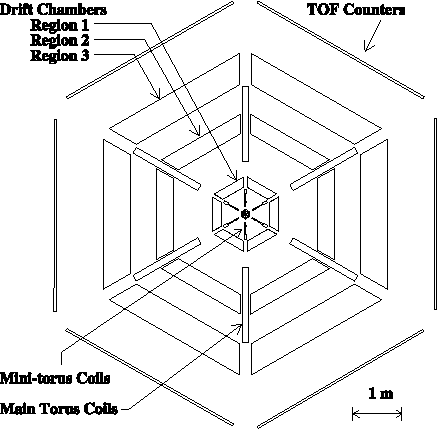
\includegraphics[width=\textwidth]{figures/CLAS_headon.pdf}
        \caption{CLAS6 as seen along the beam axis.}
    \end{subfigure}
    \hfill
    \begin{subfigure}[b]{0.5\textwidth}
        \centering
        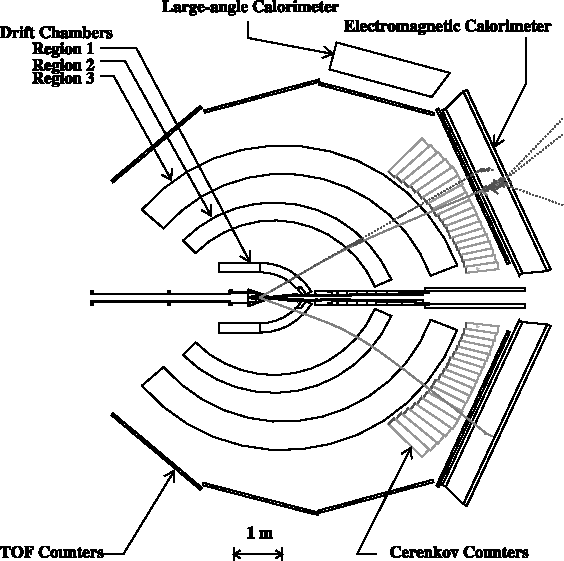
\includegraphics[width=\textwidth]{figures/CLAS_side.pdf}
        \caption{Side view cross section through the detector.}
    \end{subfigure}
    \caption{\label{fig:CLAS}
        Diagrams of the CLAS6 detector from \cite{meckingCEBAFLargeAcceptance2003}, see for more detail.
        Most important for us are the EM calorimeter spanning $\theta < 50\si{\degree}$ which detects the scattered electrons and photons.
        Cherenkov counters near the axis are needed for distinguishing electrons and negative pions and the time-of-flight (TOF) detectors help distinguish protons and positive pions.
    }
\end{figure}

\subsection{CLAS6}\label{sec:CLAS6}
The CLAS6 detector, active from 1998 to 2012 when the work on CLAS12 has began, is largely built around a set of six toroidal magnets distributed along the azimuthal angle $\phi$.
These curve the trajectories of charged particles in their $\phi$ plane and allow for charged particle momentum measurements in drift chambers.
They also give rise to distinct six sectors visible in \cref{fig:CLAS} and deadspace between them from particles hitting the magnets.

Our data, from e2a, has measurement of electrons, protons, charged pions and photons (so essentially our cross sections are inclusive over all the other particles) and each event has a list of 4 momentum measurements for each detected particle.
In order to properly compare the measured data to theoretical MC data however, it is necessary to take into account that the detector only detects some of these particles based on their directions and momentum and even then there are finite probabilities for detection.
This can be done by considering all the possible undetected particles (and errors in the ones detected) and adjusting for them to produce a measurement of the true underlying physics, this is however very complicated and error prone.
Instead, if one only needs to test a particular aspect, it is much easier to degrade the MC data according to the defects and produce theoretical prediction of what the detector should see.

\begin{figure}[H]
    \centering
    \begin{subfigure}[b]{0.45\textwidth}
        \centering
        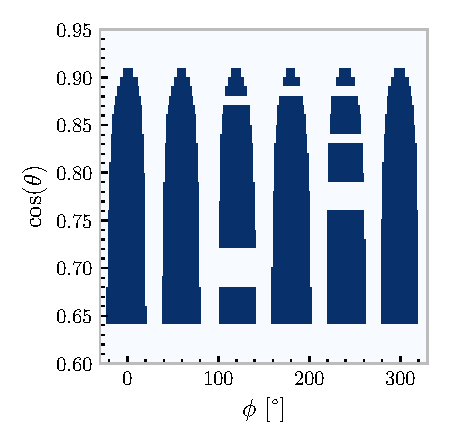
\includegraphics{figures/python/el_fid.pdf}
        \caption{$e^-$ at a momentum of 1\si{GeV}}
    \end{subfigure}
    \hspace{0.5em}
    \begin{subfigure}[b]{0.45\textwidth}
        \centering
        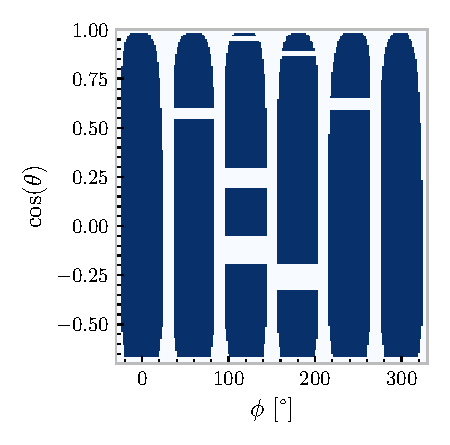
\includegraphics{figures/python/pip_fid.pdf}
        \caption{$\pi^+$ at a momentum of 0.7\si{GeV}}
    \end{subfigure}
    \caption{
        Showing the directional dependence of our fiducial cuts for data with beam energy 2.26\si{GeV}.
        The fiducials for electrons and positive pions at fixed 3 momentum magnitudes are shown, dark blue means the particle passes, grey that it is cut.
        $\phi$ angle is shown in the -30 to 330\si{\degree} range, this is in order not to cut through the accepted segment.
    }\label{fig:fid_map}
\end{figure}

\subsection{Fiducials and acceptance maps}
We do this in two steps, first we specify a fairly wide range of directions and momenta, we apply \emph{fiducial} cuts to filter these and define these as our signal in both experimental and MC data.
These reflect the harder limits of the CLAS6 detector, the precise fiducials depend on the beam energy and we have them inherited from previous \efn\ work and e2a as a collection of C\texttt{++} code, see \cite{papadopoulouLeptonNucleusScatteringMeasurements2023,mclauchlanDeltaElectroproduction12C}.
They are different for each particle type and cut on their 3 momentum size and direction, see \cref{fig:fid_map} for an example.
The six distinct zones/segments are a result of the mentioned magnets obstructing the areas in between an the gaps are due to some components not performing up to specification on the day of the experiment.
% An example is that we only consider pions with momentum over 150 \si{MeV}.

Then, if we are to truly compare MC to data, we apply \emph{acceptance} maps.
These have been compiled by e2a as well and give a probability of a particle being detected for each of the particle types and every possible direction and size of their momentum within the fiducial cuts.
These are different for each target and beam energy and are given as three dimensional histograms (\verbb{TH3F} from ROOT) with momentum magnitude, $\cos(\theta)$ and $\phi$ as the axes, see \cref{fig:acc_map}.
There probabilities are then used as weights for events when plotting histograms.

\begin{figure}[H]
    \centering
    \begin{subfigure}[b]{0.45\textwidth}
        \centering
        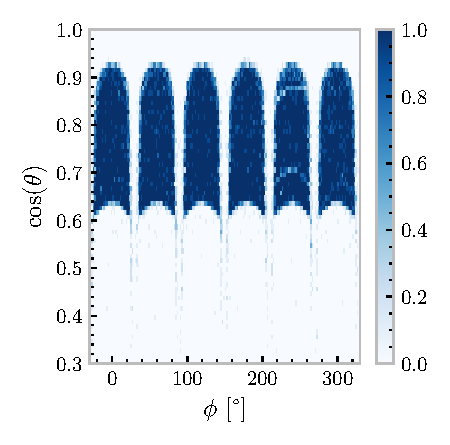
\includegraphics{figures/python/el_acc1.pdf}
        \caption{Fixed $|\vb{p}| = 1\si{GeV}$}
    \end{subfigure}
    \hspace{0.5em}
    \begin{subfigure}[b]{0.45\textwidth}
        \centering
        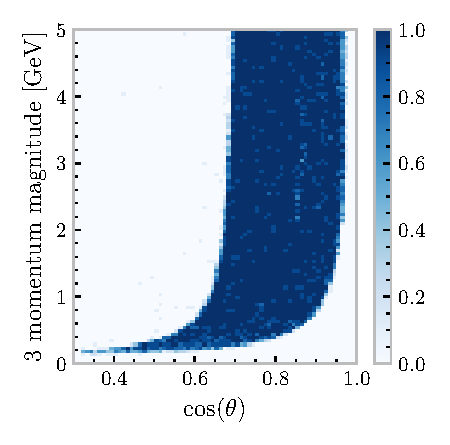
\includegraphics{figures/python/el_acc2.pdf}
        \caption{Fixed $\phi = 0$}
    \end{subfigure}
    \caption{
        Electron acceptance map projections for the 2.26\si{GeV} beam energy and C target dataset.
        The $z$, colormapped axis is the probability of an electron in the region being accepted.
    }\label{fig:acc_map}
\end{figure}

\subsection{The codebase}
These datasets are each in a ROOT file in a GENIE format called \verbb{gst}, this is a list-like object (\verbb{TTree}) of events with their properties.
As this is a GENIE format, there are fields for many properties not measured in experiments, for the CLAS6 data these are empty.
Some of the more notable fields are the outgoing electron 4 momentum, information about all the particles after the neutrino-nucleus interaction (referred to as primary or initial state) as well as the same information about post FSI particles (final state).
Some of these properties, especially the ones that never could be measured, are referred to as the `truth` as they reflect what we think is physically going on.
GENIE also adds flags to separate the QE, RES, DIS and other types of events and has information about what FSI has happened, this is described best in the GENIE manual\cite{andreopoulosGENIENeutrinoMonte2015} though it is somewhat outdated.

As there are $\sim100$ different properties per event and we have up to hundreds of millions of events, a moderately sophisticated analysis code is needed.
The main \efn\ code is available on github \cite{E4nuE4nuanalysiscodePlaceholder} as developed by Afrodite Papadopoulou, however it has since been used by various scientists each adding their own functionality.
As a result there are various versions kept by people and on github of a large, somewhat bloated and very difficult to understand code, most the logic of the analysis being in a single 4000 line file.
A main goal of this project was to redevelop and streamline this code in order to lower the entry barrier for others, make it easier to spot analysis flaws and reduce boilerplate code.

The newly developed code is also available on github \cite{kockahonzaSHPGenieData2023}, it uses C\texttt{++}17 features and ROOT 6.12 as available on the GENIE machine at Fermilab used by us.
It heavily uses classes and the features are best described by describing the code.
The main class \verbb{GenieAnalysis} will expect an input file with a \verbb{gst} dataset, has two virtual methods to be overriden \verbb{double passesCuts()} and \verbb{void useEntry(double weight)} and one method that is expected to be used \verbb{void runAnalysis(int number\_of\_entries)}\footnotemark.
\footnote{I am somewhat loose with the code for the sake of brevity, for example replacing the ROOT types with the normal C\texttt{++} ones.}
The last of which will start an analysis, it will go through the first \verbb{number\_of\_entries} events from the input file and for each \verbb{passesCuts} will be ran, its return value being used as the weight, so if it is zero that event is not used at all.
If nonzero, \verbb{useEntry(weight)} is called with that weight, this method does nothing in this class, it is expected to be overriden by inheriting classes to for example count the events, or write some properties to a histogram.
Given this structure the code is intended to provide data on the events as a whole, it is not suited for applications where some parts of an event are to accepted and some discarded.

The next and likely most useful part of the code is the \verbb{GAAutoHistograms} class, this inherits from \verbb{GenieAnalysis} and provides automatic histogram creation and filling as long as they conform to the following structure.
There are "types" and "properties" and \verbb{GAAutoHistograms} creates histograms of properties, for each type independently.
Specifically types are used to separate interaction types like QE, RES, $\Delta$ resonances and then also all events, each of these would be a type.
Properties are then the quantities of interest, like $W, Q^2$, outgoing electron momentum and angles and so on.
\verbb{GAAutoHistograms} is constructed in a way that it has a set list of "known" types and properties that can be easily added and each have a code name, the user can then specify which to use.
Specifically it can create 1D histograms for each property and type combination and also 2D histograms showing how some two properties correlate, again it can do this separately for any chosen known types.

To touch on the project structure, these and the following classes are implemented in the \verbb{GenieAnalysis} folder, then there are executables, these are \verbb{.cpp} files in the root folder which specify a given run.
For a quick summary of the rest (see \cref{fig:code_dia}), the \verbb{GACLAS6Common} file (and namespace) defines auxiliary properties specific to the CLAS6 data (like target and beam energy enumerations) and a wrapper around the original fiducials code.
The \verbb{GACLAS6MCCuts, GACLAS6MC} classes do equivalent analysis to that which the original code (as inherited from Lucas Taling, a previous MSc student) did on the GENIE data for CLAS6.
This was mainly used for first looks and testing of the new code (having five executables using these) and \verbb{GACLAS6DataPrepare, GACLAS6Data} do the equivalent for the actual CLAS6 data, though this has not been tested much.

\begin{figure}[H]
    \centering
    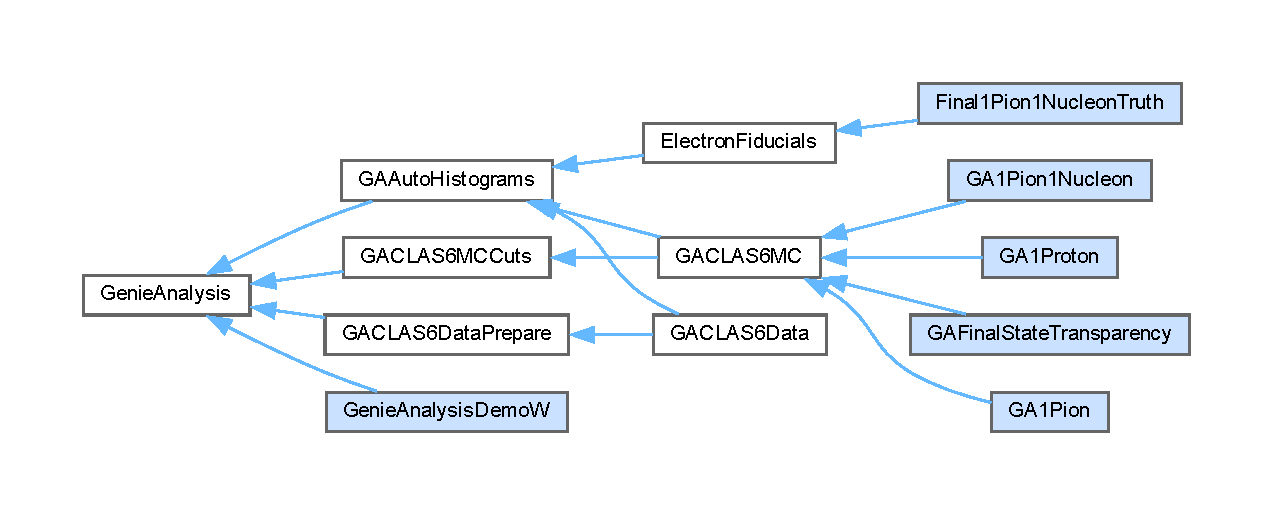
\includegraphics[width=0.9\textwidth]{figures/code_flow_diagram/diagram.pdf}
    \caption{
        A class diagram of the new code showing the relations.
        The reusable classes from the \verbb{GenieAnalysis} folder are shown with a white background, classes from executables are light blue.
    }\label{fig:code_dia}
\end{figure}


\section{Nuclear Transparency of 1 Pion 1 Nucleon Events}
Finally, once all the preliminary coding has been completed, we conduct a basic nuclear transparency study on the data.
Nuclear transparency is a very wide term describing how much of an effect do FSI have under certain conditions.
Given its nature nuclear transparency is typically studied either theoretically or from MC data as we cannot measure any particle properties before FSI.

Here we look at events with 1 charged pion 1 nucleon from a GENIE generated dataset and inspect how well we can reconstruct the pion momentum from the electron and nucleon momenta.
We use the datasets mentioned before, they are described in more detail in \cite{papadopoulouLeptonNucleusScatteringMeasurements2023}, and specifically we only look at the data with beam energy of 2.26\si{GeV} and mainly carbon target.
Importantly, GENIE was tuned to the SuSAv2 configuration using the INTRANUKE hN model for FSI (called "intranuclear transport modelling" in the GENIE documentation\cite{andreopoulosGENIENeutrinoMonte2015}).
GENIE has two models for FSI, hA and hN, the main difference being the hA modelling a hadrons path out of the nucleus as a whole, either it scatters once or not at all.
hN performs a full IntraNuclear Cascade (INC), each hadron can rescatter multiple times including hadrons produced from a previous rescattering, of the two hN is the more accurate though slower model\cite{andreopoulosGENIENeutrinoMonte2015}.

The pion reconstruction is done as for simple pion production of exactly 1 charged pion and 1 nucleon without any FSI, the main channels of this process we are looking for are the $\Delta$ resonance showed in \cref{fig:RESel_fd}.
We then further assume the struck nucleon to be at rest and the reconstruction goes as described below and shown in \cref{eq:reco_ass,eq:reco_res}.
Denoting the 4 momenta of the electron and nucleon before collision as $q_e^\mu$ and $q_n^\mu$, both of which we know.
Their sum must be equal to the sum of the 4 momenta of the outgoing electron, pion and nucleon, denoted respectively as $p_e^\mu, p_\pi^\mu$ and $p_n^\mu$.

\begin{align}\label{eq:reco_ass}
    q_e^\mu &\leftrightarrow \begin{pmatrix} E_b \\ \sqrt{E_b^2 - m_e^2} \\ 0 \\ 0 \end{pmatrix} &
    q_n^\mu &\sim \begin{pmatrix} m_n \\ 0 \\ 0 \\ 0 \end{pmatrix}
\end{align}
\begin{align}\label{eq:reco_res}
    q_i^\mu + q_n^\mu &= p_e^\mu + p_\pi^\mu + p_n^\mu \implies \nonumber \\
    p_\pi^\mu &= q_i^\mu + q_n^\mu - p_e^\mu - p_n^\mu
\end{align}

Of course for the data this will rarely work perfectly, we expect 3 main sources of errors -- the original nucleon having nonzero momentum, other pion production processes producing other undetected particles, mainly other resonances and DIS, (photons, other mesons\ldots) and finally FSI.
However they all have different signatures and so we can largely separate them, first we however need to define our signal.

We have conducted many runs with different parameters, they can be summarized by three options, which event set we use, which combination of charged pion and nucleon we are looking for and if we do a cut on $W$.
The event sets and $W$ cut are described below and the pion/nucleon combination is fairly self-explanatory.
Data for all 4 of these combinations was collected though as they are largely the same we focus on $1\pi^-1p$ events as this is the only combination produced by $\Delta$ resonances that we have fiducials and acceptances for both of the particles.
% The pion/nucleon combination is fairly self-explanatory and data was collected for all four combinations, the other options are described below.
% The pion/nucleon combination is fairly self-explanatory, the event sets are described below and the W cut refers to us only using events with an invariant hadronic mass of $< 1.4\si{GeV}$.
% This is in order to maximize the fraction of $\Delta$ resonant events we get and is justified later.

\subsection{The event sets}
The 4 different event sets are the Primary State (PS), Final State with no Rescattering (FSR), any Final State (FS) and Detector Like (DL) runs.
For all of them we use the CLAS6 fiducial cuts, for PS, FSR and FS the first part is the same, we check if the electron 3 momentum passes the fiducial cuts and the event is only used if it does.

\paragraph{Primary State (PS)} is the closest to the "truth"/physics we get here.
After checking the electron fiducials, particle data from the GENIE reported primary state (GENIE label, means before FSI) is used.
The code then goes through all the produced hadrons and only charged pions and protons that pass their fiducials are considered, along with all neutrons (we don't have fiducials for them as they weren't detected in the e2a CLAS6 data).
Only if there are exactly 1 charged pion and 1 nucleon of the required types and 0 of the others, is the event used.
Notably there is another way the fiducials could be applied, we could only consider event where all charged pions and protons pass their fiducials and only then check their numbers.
This method was also tried and resulted in near identical results and so it suggests the decision isn't a major one.

\paragraph{Final State with no Rescattering (FSR)} should in theory and we observe it to be almost the same as PS.
GENIE also reports for each particle in the primary state a \verbb{resc} code specifying if and in what way did that primary state particle rescatter in FSI.
In FSR the final state (means post FSI) particle properties and 3 momenta are used, however only events where all the \verbb{resc} codes indicated no rescattering.
The final state particles are then processed in the same way as in PS, only particles passing fiducials are considered and the counts of charged pions and nucleons must exactly match.

\paragraph{Final State (FS)} means we use final state particles and their properties just as in FSR, but do no checking of \verbb{resc}.
This should result in increased noise and for example getting pion plus nucleon events even from QE scattering as they can be produced in FSI.

\paragraph{Detector Like (DL)} This is to get some insight into what level of precision we might expect from detector data.
This event set introduces an additional element of Monte Carlo methods, starting with the electron, if it passes the fiducial cuts its acceptance is calculated.
Then according to the acceptance likelihood it is randomly either accepted or rejected, if accepted the 3 momentum magnitude will be smeared in the same way that previous \efn\ work has used.
This is done by drawing a number from a Gaussian distribution with mean of the original distribution and $\sigma$ of 0.005 times the original magnitude.

Then for the hadron particles, we use particle from the final state that pass their fiducial cuts.
Then as in our case neutrons aren't detected they are taken at this stage, however for charged pions and protons their acceptances are calculated and are either accepted or rejected randomly according to them in the same way as electron.
Their 3 momenta are then also smeared in the same way this time using 0.007 for charged pions and 0.01 for protons as the scaling factor for $\sigma$.

\begin{figure}[H]
    \centering
    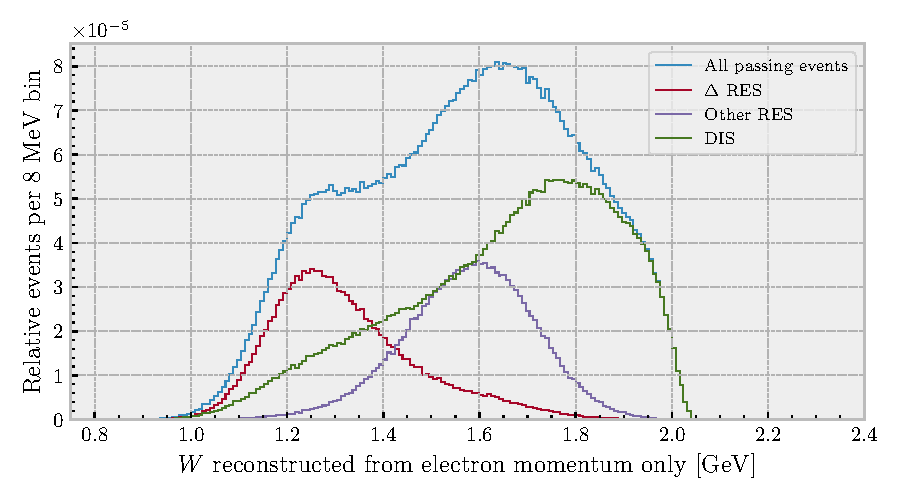
\includegraphics{figures/python/W_demo.pdf}
    \caption{
        $W$ distribution for the PS, 1$\pi^-1p$ event set without the $W$ cut, there are no QE events as they never produce pions before FSI.
        The relative number of events is the number of passing events in the bin divided by all the events in the dataset ($\sim$175 million) before any fiducials.
        Carbon target and 2.26\si{GeV} beam energy.
    }\label{fig:W_demo}
\end{figure}

\subsection{The $W$ cut}
This is an extra cut to try to separate the $\Delta$ resonances using only properties known to experiments.
Also note that again assuming the struck nucleon being at rest\footnotemark\ we can calculate $W^2 = r_\mu r^\mu = (q_e^\mu + q_n^\mu - p_e^\mu)^2$ and so reconstruct $W$ solely from the electron 4 momentum.
\footnotetext{This method for $W$ reconstruction is often used (GENIE calculates such a value) though even if it was incorrect in terms of being equal to the hadronic invariant mass, its use as a cut still holds.}
\Cref{fig:W_demo} shows a histogram of the electron reconstructed $W$ values for one of the runs split by different interaction types, similar plots are often produced by studies.
As we have selected only pre FSI pion production events there are no QE events, otherwise they would form a narrow peak near 1\si{GeV}.
The peak of the non-$\Delta$ resonances corresponds to the $N$ mass and DIS events typically come in behind them and with a sharp drop off near 2\si{GeV} as the incident electrons have energy 2.26\si{GeV}.
If we then only consider events in some range of $W$ values we can change the relative dominance of the interaction types.

This process can of course be done with any event property, we choose $W$ as previous work by Lucas Taling in his MSc thesis has shown that it is the ideal choice for separating $\Delta$ resonances.
We then choose the optimal cut value by considering purity, the number of passing $\Delta$ events over all passing events, and efficiency, the number of passing $\Delta$ events over all $\Delta$ events.
\Cref{fig:W_cut_metr} shows a sample plot of these quantities along with their product which we choose as our metric for choosing the cut.
Only one such plot is shown, but all the others are very similar and give values of $1.4 \pm 0.02 \si{GeV}$ for the optimal cut thus we use 1.4\si{GeV}.

\begin{figure}[H]
    \centering
    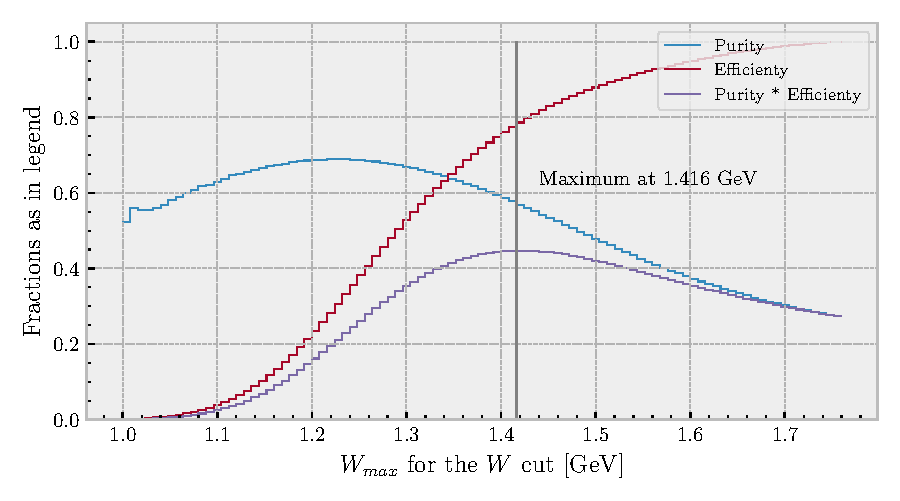
\includegraphics{figures/python/W_cut_metr.pdf}
    \caption{
        The performance of the $W$ cut for the PS, $1\pi^-1p$ no $W$ cut event set, purity and efficiency as defined above in text.
        Numbers are calculated directly from the $W$ histogram, hence the steps.
        Carbon target and 2.26\si{GeV} beam energy.
    }\label{fig:W_cut_metr}
\end{figure}

\subsection{Primary state results}
The first useful quantities come from the PS run where we can also check the \verbb{resc} codes of the pion and nucleon and see how often they do rescatter in FSI.
See \cref{tab:FSI_re} for these results, these are plausible within other literature numbers, \cite{stevendytmanFinalStateInteractions2009} quotes a 20\% chance of a pion being absorbed in a carbon nucleus.
In our data we see 20\% and 21\% for \md\ and \pd\ respectively, other rescattering mechanisms accounting for the rest.

\begin{table}[H]
    \begin{center}
        \begin{tabular}{ c | c | c }
            & \md & \pd \\
            \hline
            \% of events with no $\pi$ rescatter & 63.9 & 61.8 \\  
            \hline
            \% of events with no nucleon rescatter & 77.7 & 74.3 \\
        \end{tabular}
    \end{center}
    \caption{FSI rescattering rates for PS event sets without $W$ cut, of carbon target at beam energy 2.26\si{GeV}.}\label{tab:FSI_re}
\end{table}

\begin{figure}[H]
    \centering
    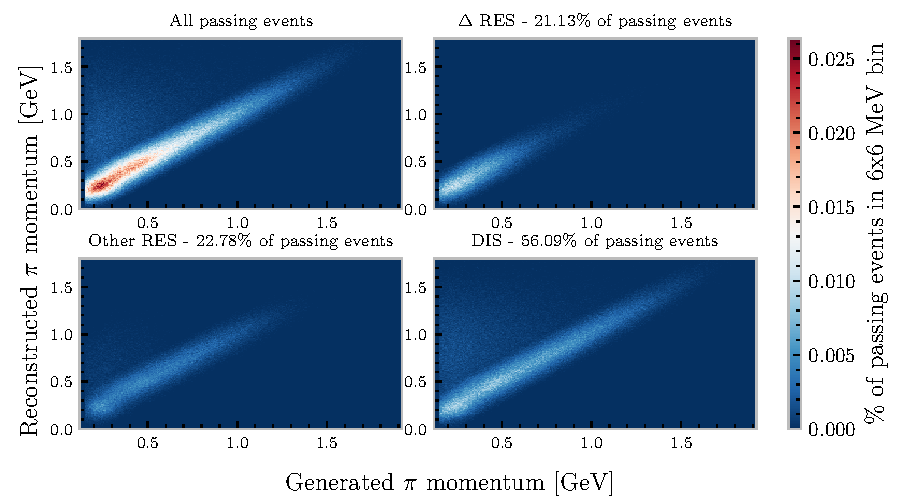
\includegraphics{figures/python/vs_pp_C_m_ps.pdf}
    \caption{
        Correlation of actual and reconstructed pion momentum magnitude for the \md, PS, no $W$ cut data.
        The $\Delta$ events have a near constant width due to the original nucleon nonzero momentum and no off diagonal events.
        Other resonant events and DIS both have the same width and also off diagonal events as they will more commonly produce other unaccounted for particles including photons and mesons.
        Carbon target and 2.26\si{GeV} beam energy.
    }\label{fig:vs_pp_ps1}
\end{figure}

For a qualitative look at the pion momentum reconstruction performance, 2D histograms of events with respect to actual and reconstructed pion momentum magnitude are the most useful (such plots for $\cos(\theta)$ and $\phi$ were generated but didn't show anything interesting).
\Cref{fig:vs_pp_ps1,fig:vs_pp_ps2} show these for the PS, \md\ and \pd\ event sets.
Also note that there is no separate diagram for QE events, for PS and FSR event sets there are none as pions are only created in FSI for QE events.
Some QE events did appear for FS and DL event sets however at most 1\% (see \cref{fig:extra1} in \cref{app:extra}) and only constitute noise.

The main difference between \cref{fig:vs_pp_ps1,fig:vs_pp_ps2} is that the \pd\ has more events and less of the events are from $\Delta$ resonances.
This shows that the fiducials already significantly help separating other resonant and especially DIS events.
The main result from both is that all $\Delta$ events are distributed along the diagonal, meaning the reconstruction works as it should with the width being due to the nonzero struck nucleon momentum\footnotemark, an initial state effect and showing this can act a probe of nuclear structure.
\footnotetext{The fact that visually the width seems to decrease is just an effect from there being less events at higher momenta.}

Finally, the FSR event set should yield exactly the same event properties as PS except it will not accept any where rescattering later occurred.
As such the same plots are shown in \cref{app:extra}, \cref{fig:vs_pp_fsr}, the only notable difference being a significant drop in event counts near pion momentum $\sim 270\si{MeV}$.
This is points to pions or nucleons experiencing an increase in FSI interactions near the area and also shows up in FS and DL data.

\begin{figure}[H]
    \centering
    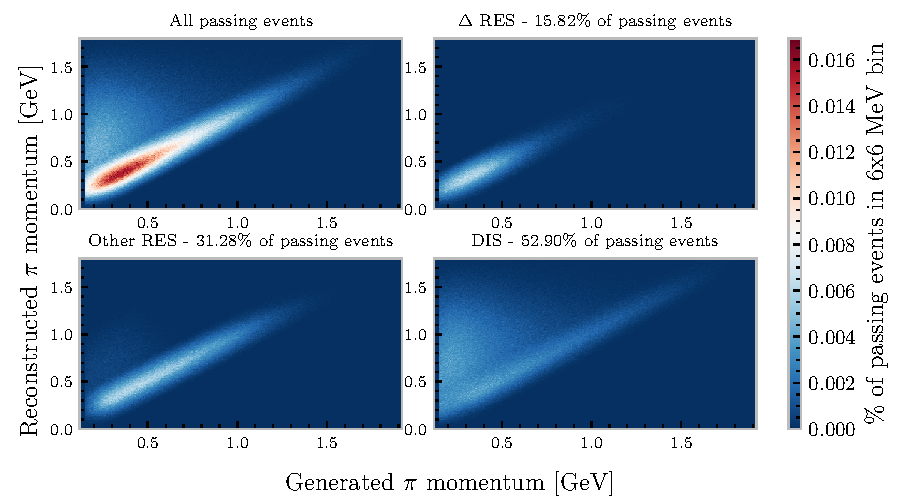
\includegraphics{figures/python/vs_pp_C_p_ps.pdf}
    \caption{
        Correlation of actual and reconstructed pion momentum magnitude for the \md, PS, no $W$ cut data.
        Same observations apply as to \cref{fig:vs_pp_ps1} though are many more events here due to the lack of fiducials for $n$.
        Carbon target and 2.26\si{GeV} beam energy.
    }\label{fig:vs_pp_ps2}
\end{figure}

\subsection{Detector like and other results}
Moving on to data more likely to reflect experiment, FS and DL show similar features and no other differences between \md\ and \pd\ than that pointed out before appear so I only focus on the DL, \md\ event set.
Without the $W$ cut we get similar results as in \cref{fig:vs_pp_ps1} but with added noise and the mentioned lack of events near pion momentum of 270\si{MeV}, notably however only 16\% of the events are $\Delta$ resonances and 64\% are very noisy DIS events.
The post $W$ data is shown in \cref{fig:vs_pp_dl_W} \ldots yadada \ldost tomorrow morning

\begin{figure}[H]
    \centering
    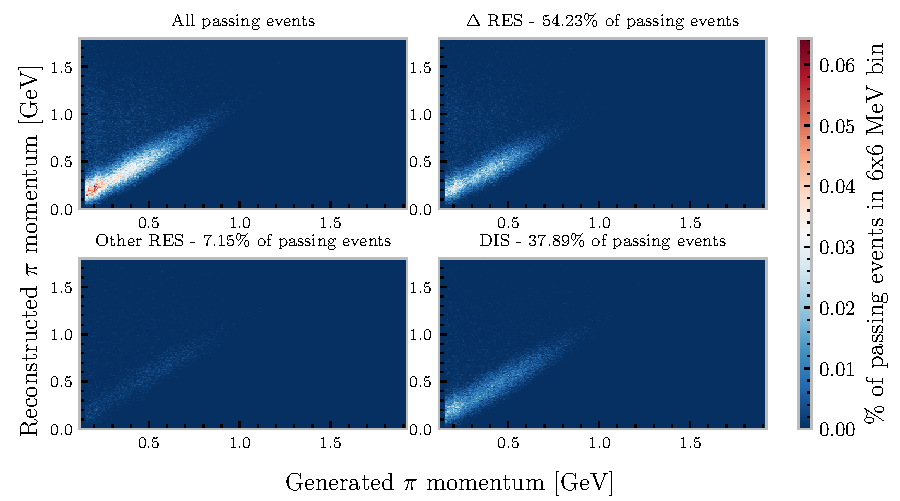
\includegraphics{figures/python/vs_pp_C_m_dl_W.pdf}
    \caption{
        Correlation of actual and reconstructed pion momentum magnitude for the \md, DL, data with the $W$ cut applied.
        Carbon target and 2.26\si{GeV} beam energy.
    }\label{fig:vs_pp_dl_W}
\end{figure}


Another metric worth inspecting is the actual an reconstructed pions 3 momentum magnitude difference, call it $\Delta p = |\vb{p}_{reco}| - |\vb{p}_{actual}|$.
While it could be somewhat misleading in terms of us subtracting magnitudes of vectors as opposed to getting the magnitude of the vector difference.
However the direction reconstruction performs to a similar degree as the magnitude (see \cref{app:extra,fig:vs_dir_dl}) and so the two vectors are in a similar direction.
Overall this number provides a good qualitative metric of how good the reconstruction is.
isn't fully explained yet but the plot is showing in out most "detector like" setup we can reconstruct it to within ~400MeV for most events.

\begin{figure}[H]
    \centering
    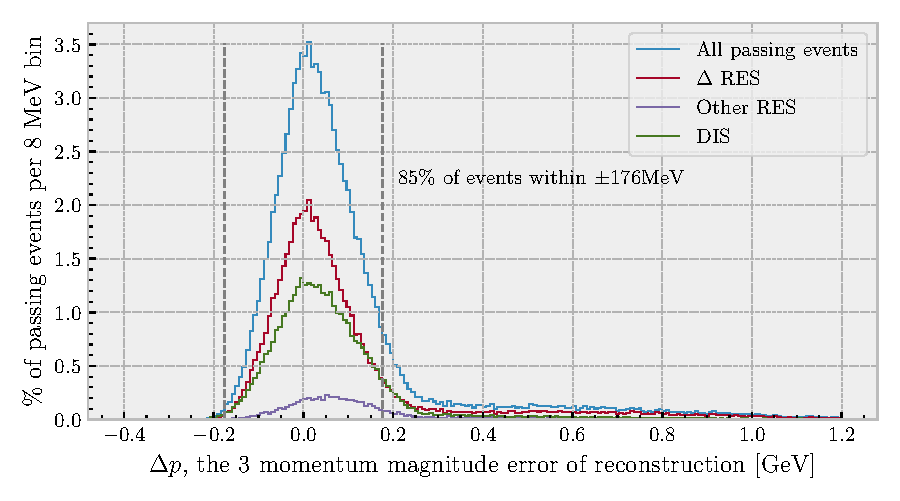
\includegraphics{figures/python/metr_m_dl_W.pdf}
    \caption{
        % Correlation of actual and reconstructed pion momentum magnitude for the \md, DL, data with the $W$ cut applied.
        Carbon target and 2.26\si{GeV} beam energy.
    }\label{fig:p_test_dl_W}
\end{figure}


\newpage

\printbibliography

\newpage

\begin{appendices}
    \section{Additional Data and Plots}\label{app:extra}
    \begin{table}[H]
        \begin{center}
            \begin{tabular}{ c | c | c | c | c | c | c }
                $\pi$, nucleon & Event set & Uses $W$ cut & QE [\%] & $\Delta_{1232}$ RES [\%] & Other RES [\%] & DIS [\%] \\
                \hline
                $1\pi^-1p$ & PS & no & 0.00 & 21.13 & 22.78 & 56.09 \\
                $1\pi^-1p$ & PS & yes & 0.00 & 59.36 & 8.28 & 32.36 \\
                $1\pi^-1p$ & FSR & no & 0.00 & 14.30 & 18.25 & 67.45 \\
                $1\pi^-1p$ & FSR & yes & 0.00 & 50.51 & 6.41 & 43.08 \\
                $1\pi^-1p$ & FS & no & 0.18 & 16.49 & 20.54 & 62.78 \\
                $1\pi^-1p$ & FS & yes & 0.72 & 54.21 & 6.97 & 38.09 \\
                $1\pi^-1p$ & DL & no & 0.16 & 15.71 & 20.52 & 63.59 \\
                $1\pi^-1p$ & DL & yes & 0.71 & 54.23 & 7.15 & 37.89 \\
                $1\pi^+1n$ & PS & no & 0.00 & 15.82 & 31.28 & 52.90 \\
                $1\pi^+1n$ & PS & yes & 0.00 & 55.06 & 17.80 & 27.14 \\
                $1\pi^+1n$ & FSR & no & 0.00 & 12.87 & 26.47 & 60.66 \\
                $1\pi^+1n$ & FSR & yes & 0.00 & 49.93 & 15.34 & 34.73 \\
                $1\pi^+1n$ & FS & no & 0.20 & 13.02 & 27.59 & 59.19 \\
                $1\pi^+1n$ & FS & yes & 1.00 & 50.47 & 15.51 & 33.02 \\
                $1\pi^+1n$ & DL & no & 0.12 & 12.06 & 30.67 & 57.16 \\
                $1\pi^+1n$ & DL & yes & 0.69 & 51.53 & 18.98 & 28.80
            \end{tabular}
        \end{center}
        \caption{
            Shows how many of each presented type of events there were in each data run for \md\ and \pd runs.
            The percentages are of all passing events from the run so they don't necessarily have to add to 100\% if any other unmentioned types occurred, however from these the minimum was 99.987\% meaning our select types of events are very close to covering all occurring types.
        }\label{fig:extra1}
    \end{table}

    \begin{figure}[H]
        \centering
        \begin{subfigure}{\textwidth}
            \centering
            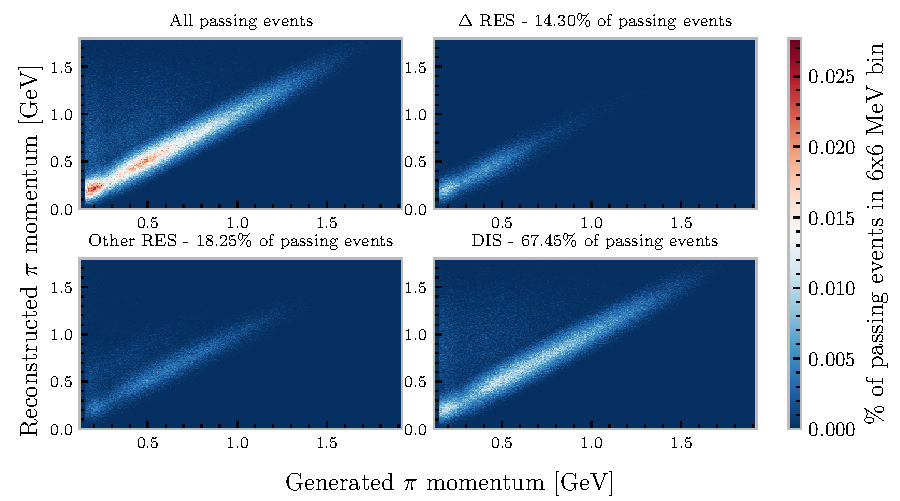
\includegraphics{figures/python/vs_pp_C_m_fsr.pdf}
            \caption{\md\ event set}
        \end{subfigure}
        \\
        \begin{subfigure}{\textwidth}
            \centering
            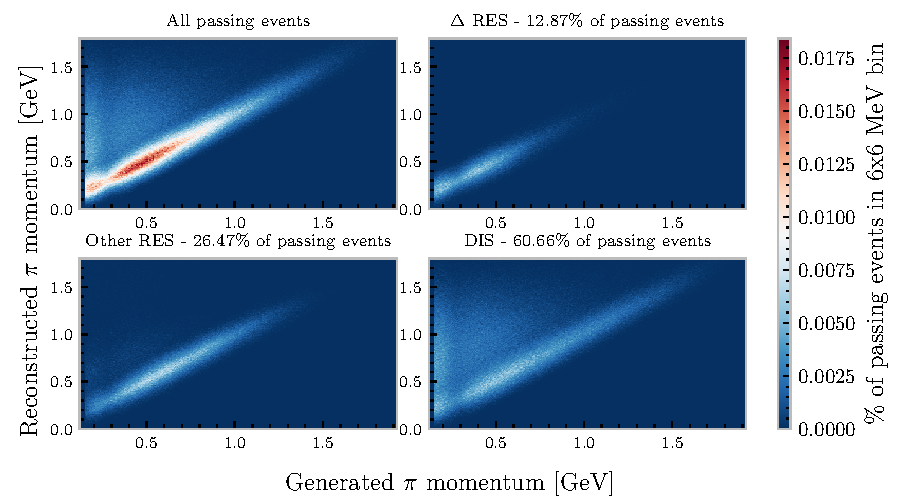
\includegraphics{figures/python/vs_pp_C_p_fsr.pdf}
            \caption{\pd\ event set}
        \end{subfigure}{\textwidth}
        \caption{
            Correlation of actual and reconstructed pion momentum magnitude for the FSR, no $W$ cut data.
            Both similar to their counterparts \cref{fig:vs_pp_ps1,fig:vs_pp_ps2} with a notable difference being a gap at actual pion momentum near 270\si{MeV}.
            This points to FSI being prominent at these momenta as the only difference between PS and FSR event sets is that events with FSI will not be present in FSR.
            Data to test this specifically however was not collected.
            Carbon target and 2.26\si{GeV} beam energy.
        }\label{fig:vs_pp_fsr}
    \end{figure}

    \begin{figure}[H]
        \centering
        \begin{subfigure}{\textwidth}
            \centering
            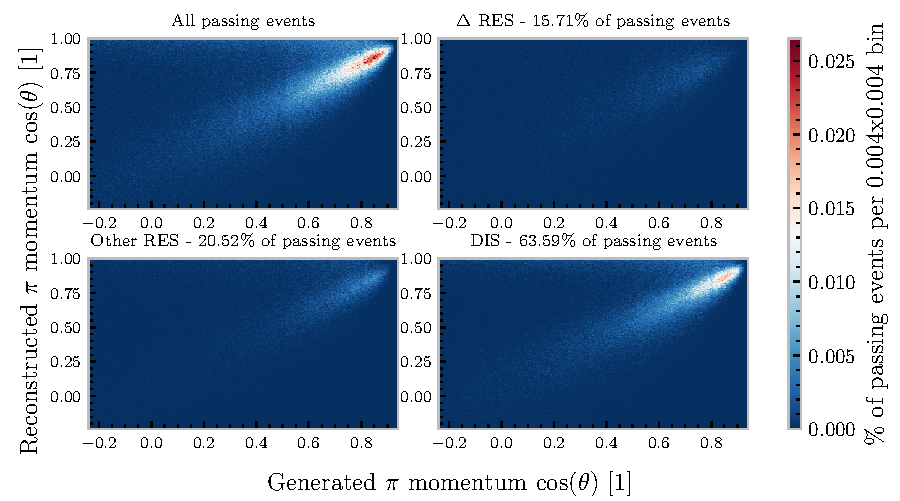
\includegraphics{figures/python/vs_ct_C_m_dl.pdf}
            \caption{$\cos(\theta)$ reconstruction performance}
        \end{subfigure}
        \\
        \begin{subfigure}{\textwidth}
            \centering
            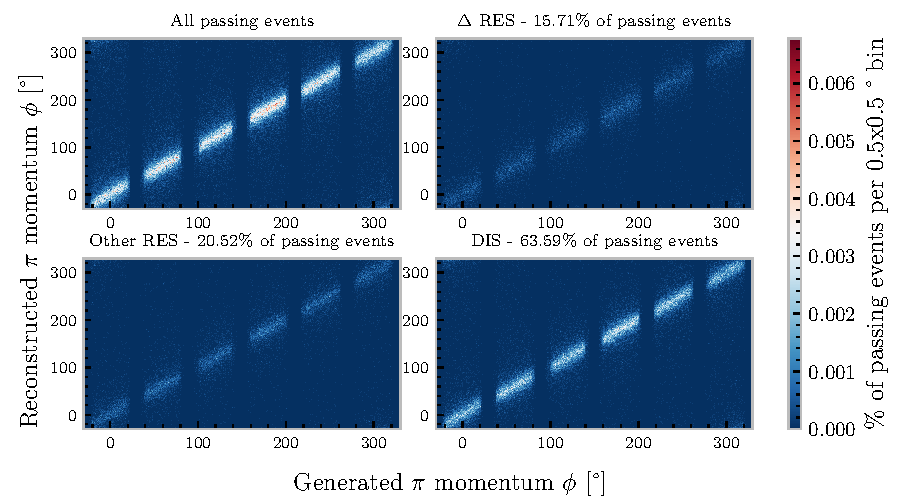
\includegraphics{figures/python/vs_phi_C_m_dl.pdf}
            \caption{$\phi$ reconstruction performance}
        \end{subfigure}{\textwidth}
        \caption{
            Performance of the directional part of pion 3 momentum reconstruction for the DL, \md, no $W$ cut data.
            Other event sets performed very similarly.
            The $\phi$ plot clearly shows how only pions passing the fiducials cuts are accepted (showing the 6 sectors from \cref{sec:CLAS6}).
            The "flare" going left and slightly up from the dominant cluster of events in the $\cos(\theta)$ is likely due to not true \md events with undetected particles.
            Carbon target and 2.26\si{GeV} beam energy.
        }\label{fig:vs_dir_dl}
    \end{figure}


\end{appendices}

\end{document}
